\chapter[Sprint IV]{Study and Implementation of Sprint IV: Diagram \& Workspace Management}

\minitoc

\section{Introduction}
Sprint IV focuses on the core functionality of diagram and workspace management within our application. This sprint represents a significant milestone in developing a comprehensive diagramming tool that enables users to create, manage, and interact with diagrams efficiently. The implementation includes both diagram lifecycle management and advanced workspace features such as AI-assisted editing and interactive code editing capabilities.

\section{Sprint Planning}

\subsection{Objectives of Sprint IV}
The primary objectives of Sprint IV are to implement comprehensive diagram management capabilities and establish a robust workspace environment that enhances user productivity. Key goals include enabling users to perform full CRUD operations on diagrams, implementing an interactive workspace with split-view functionality, integrating AI assistance for diagram editing, and establishing seamless integration with PlantUML server for diagram rendering.

\subsection{Backlog of Sprint IV}
\begin{table}[H]
\centering
\caption{Sprint IV Backlog}
\begin{tabular}{|c|l|c|l|c|}
\hline
\textbf{Epic} & \textbf{Feature} & \textbf{ID} & \textbf{User Story} & \textbf{Priority} \\
\hline
\multirow{5}{*}{4} & \multirow{5}{*}{Manage Diagrams} & 4.1 & As a user; I want to create a new diagram so that I can visualize my ideas. & M \\
\cline{3-5}
& & 4.2 & As a user; I want to view my diagram so that I can review my work. & M \\
\cline{3-5}
& & 4.3 & As a user; I want to update diagram details so that I can improve my designs. & M \\
\cline{3-5}
& & 4.4 & As a user; I want to delete a diagram so that I can remove unwanted content. & M \\
\cline{3-5}
& & 4.5 & As a user; I want to download diagram images in appropriate formats so that I can use them in other applications. & S \\
\hline
\multirow{5}{*}{5} & \multirow{5}{*}{Manage Workspace} & 5.1 & As a user; I want to control and split views in my workspace so that I can work efficiently. & S \\
\cline{3-5}
& & 5.2 & As a user; I want to edit diagram code in an interactive editor so that I can create diagrams efficiently. & M \\
\cline{3-5}
& & 5.3 & As a user; I want to chat with an AI model to edit diagram code so that I can get assistance with complex diagrams. & C \\
\cline{3-5}
& & 5.4 & As an AI system; I need to respond to user requests and help edit diagram code so that users can create better diagrams. & C \\
\cline{3-5}
& & 5.5 & As a PlantUML Server; I need to render diagram code into diagram images so that users can visualize their work. & M \\
\hline
\end{tabular}
\end{table}

\section{Analyse}

\subsection{Use case diagram for sprint IV}
The use case diagram for Sprint IV illustrates the interaction between different actors and the system functionalities. The diagram encompasses both diagram management and workspace management features, showing how users interact with the system to create, manage, and edit diagrams while leveraging AI assistance and PlantUML rendering capabilities.

\begin{figure}[H]
\centering
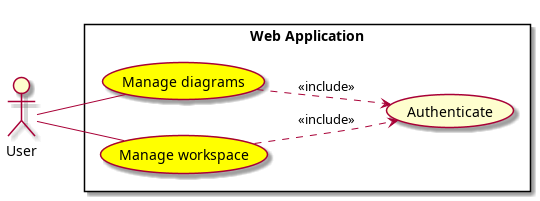
\includegraphics[width=0.8\textwidth]{conception/SprintIV/use_case_diagrams/use_case_diagram_of_SprintIV.png}
\caption{Use Case Diagram of Sprint IV}
\end{figure}

\subsection{Refined use case "Manage Diagrams"}

\begin{figure}[H]
\centering
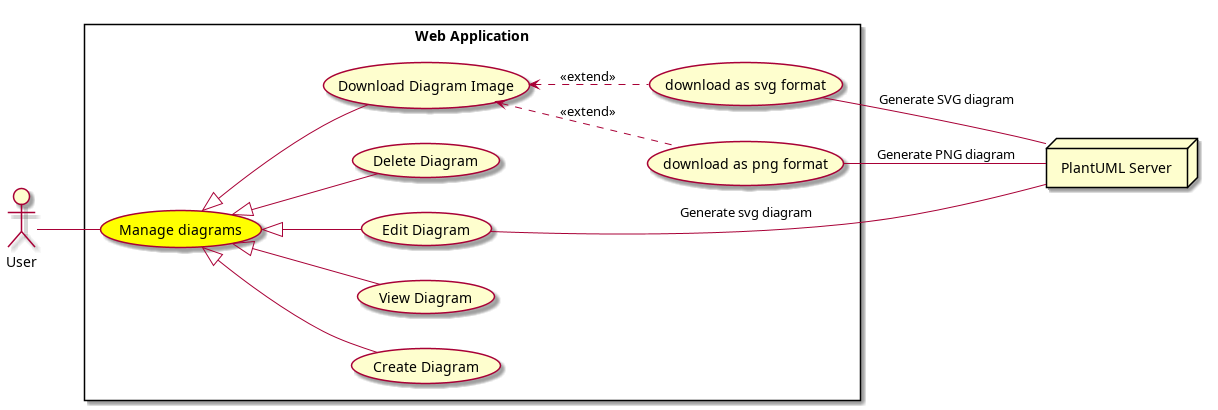
\includegraphics[width=0.8\textwidth]{conception/SprintIV/use_case_diagrams/refined_use_case_feature_diagram_management.png}
\caption{Refined Use Case - Manage Diagrams}
\end{figure}

\subsubsection{Use case}
\begin{verbatim}
usecase "Create Diagram" as CreateDiagram
usecase "View Diagram" as ViewDiagram  
usecase "Delete Diagram" as DeleteDiagram
\end{verbatim}

\subsubsection{Textual description of use case "Create new diagram"}
\begin{table}[H]
\centering
\caption{Use Case Description - Create New Diagram}
\begin{tabular}{|l|p{10cm}|}
\hline
\textbf{Use Case Name} & Create New Diagram \\
\hline
\textbf{Actor} & User \\
\hline
\textbf{Description} & This use case allows a user to create a new diagram in the system \\
\hline
\textbf{Preconditions} & User is authenticated and has access to the application \\
\hline
\textbf{Postconditions} & A new diagram is created and saved in the system \\
\hline
\textbf{Main Flow} & 1. User clicks on "Create New Diagram" button \\
& 2. System displays diagram creation form \\
& 3. User enters diagram name and selects diagram type \\
& 4. User clicks "Create" button \\
& 5. System validates input and creates new diagram \\
& 6. System redirects user to diagram editor with new diagram \\
\hline
\textbf{Alternative Flow} & 3a. User enters invalid or duplicate diagram name \\
& 3a1. System displays error message \\
& 3a2. Return to step 3 \\
\hline
\textbf{Exceptions} & System error during diagram creation \\
\hline
\end{tabular}
\end{table}

\subsubsection{Textual description of use case "View diagram"}
\begin{table}[H]
\centering
\caption{Use Case Description - View Diagram}
\begin{tabular}{|l|p{10cm}|}
\hline
\textbf{Use Case Name} & View Diagram \\
\hline
\textbf{Actor} & User \\
\hline
\textbf{Description} & This use case allows a user to view an existing diagram \\
\hline
\textbf{Preconditions} & User is authenticated and diagram exists in the system \\
\hline
\textbf{Postconditions} & Diagram is displayed to the user \\
\hline
\textbf{Main Flow} & 1. User selects a diagram from the diagram list \\
& 2. System retrieves diagram data \\
& 3. System renders diagram using PlantUML server \\
& 4. System displays rendered diagram to user \\
\hline
\textbf{Alternative Flow} & 2a. Diagram data is corrupted or missing \\
& 2a1. System displays error message \\
& 2a2. User is redirected to diagram list \\
\hline
\textbf{Exceptions} & PlantUML server unavailable, Network connectivity issues \\
\hline
\end{tabular}
\end{table}

\subsubsection{Textual description of use case "Delete diagram"}
\begin{table}[H]
\centering
\caption{Use Case Description - Delete Diagram}
\begin{tabular}{|l|p{10cm}|}
\hline
\textbf{Use Case Name} & Delete Diagram \\
\hline
\textbf{Actor} & User \\
\hline
\textbf{Description} & This use case allows a user to delete an existing diagram \\
\hline
\textbf{Preconditions} & User is authenticated and diagram exists in the system \\
\hline
\textbf{Postconditions} & Diagram is permanently removed from the system \\
\hline
\textbf{Main Flow} & 1. User selects a diagram to delete \\
& 2. User clicks "Delete" button \\
& 3. System displays confirmation dialog \\
& 4. User confirms deletion \\
& 5. System removes diagram from database \\
& 6. System updates diagram list view \\
\hline
\textbf{Alternative Flow} & 4a. User cancels deletion \\
& 4a1. System closes confirmation dialog \\
& 4a2. No changes are made \\
\hline
\textbf{Exceptions} & Database error during deletion \\
\hline
\end{tabular}
\end{table}

\subsection{Refined use case "Manage Workspace"}

\begin{figure}[H]
\centering
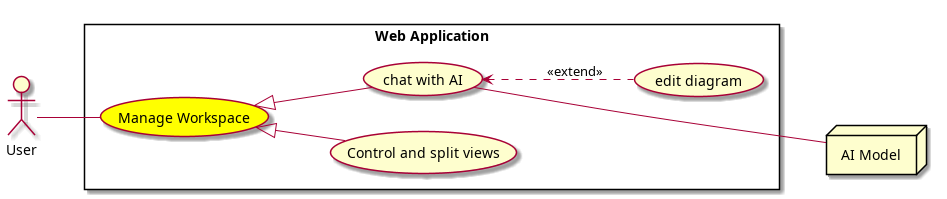
\includegraphics[width=0.8\textwidth]{conception/SprintIV/use_case_diagrams/refined_use_case_feature_workspace_management.png}
\caption{Refined Use Case - Manage Workspace}
\end{figure}

\subsubsection{Textual description of use case "load workspace"}
\begin{table}[H]
\centering
\caption{Use Case Description - Load Workspace}
\begin{tabular}{|l|p{10cm}|}
\hline
\textbf{Use Case Name} & Load Workspace \\
\hline
\textbf{Actor} & User \\
\hline
\textbf{Description} & This use case allows a user to load their workspace with existing diagrams and settings \\
\hline
\textbf{Preconditions} & User is authenticated \\
\hline
\textbf{Postconditions} & Workspace is loaded with user's diagrams and preferences \\
\hline
\textbf{Main Flow} & 1. User accesses the application \\
& 2. System authenticates user \\
& 3. System retrieves user's workspace data \\
& 4. System loads diagram list and workspace layout \\
& 5. System displays workspace to user \\
\hline
\textbf{Alternative Flow} & 3a. No existing workspace data found \\
& 3a1. System creates default workspace \\
& 3a2. Continue with step 4 \\
\hline
\textbf{Exceptions} & Database connectivity issues, Authentication failure \\
\hline
\end{tabular}
\end{table}

\subsubsection{Textual description of use case "chat with AI"}
\begin{table}[H]
\centering
\caption{Use Case Description - Chat with AI}
\begin{tabular}{|l|p{10cm}|}
\hline
\textbf{Use Case Name} & Chat with AI \\
\hline
\textbf{Actor} & User \\
\hline
\textbf{Description} & This use case allows a user to interact with AI assistant for diagram editing help \\
\hline
\textbf{Preconditions} & User is in workspace with active diagram, AI service is available \\
\hline
\textbf{Postconditions} & User receives AI assistance for diagram editing \\
\hline
\textbf{Main Flow} & 1. User opens AI chat panel \\
& 2. User types question or request about diagram \\
& 3. System sends request to AI service \\
& 4. AI processes request and generates response \\
& 5. System displays AI response to user \\
& 6. User can apply suggested changes to diagram \\
\hline
\textbf{Alternative Flow} & 3a. AI service is unavailable \\
& 3a1. System displays service unavailable message \\
\hline
\textbf{Exceptions} & AI service timeout, Network connectivity issues \\
\hline
\end{tabular}
\end{table}

\subsubsection{Textual description of use case "clear chat"}
\begin{table}[H]
\centering
\caption{Use Case Description - Clear Chat}
\begin{tabular}{|l|p{10cm}|}
\hline
\textbf{Use Case Name} & Clear Chat \\
\hline
\textbf{Actor} & User \\
\hline
\textbf{Description} & This use case allows a user to clear the chat history with AI assistant \\
\hline
\textbf{Preconditions} & User has an active chat session with AI \\
\hline
\textbf{Postconditions} & Chat history is cleared and conversation is reset \\
\hline
\textbf{Main Flow} & 1. User clicks "Clear Chat" button \\
& 2. System displays confirmation dialog \\
& 3. User confirms action \\
& 4. System clears chat history \\
& 5. System resets chat interface \\
\hline
\textbf{Alternative Flow} & 3a. User cancels action \\
& 3a1. System closes confirmation dialog \\
& 3a2. Chat history remains unchanged \\
\hline
\textbf{Exceptions} & None \\
\hline
\end{tabular}
\end{table}

\subsubsection{Textual description of use case "edit diagram"}
\begin{table}[H]
\centering
\caption{Use Case Description - Edit Diagram}
\begin{tabular}{|l|p{10cm}|}
\hline
\textbf{Use Case Name} & Edit Diagram \\
\hline
\textbf{Actor} & User \\
\hline
\textbf{Description} & This use case allows a user to edit diagram code in the interactive editor \\
\hline
\textbf{Preconditions} & User has selected a diagram and is in workspace \\
\hline
\textbf{Postconditions} & Diagram code is modified and preview is updated \\
\hline
\textbf{Main Flow} & 1. User opens diagram in editor \\
& 2. System displays diagram code in editor panel \\
& 3. User modifies diagram code \\
& 4. System automatically renders preview \\
& 5. User reviews changes in preview panel \\
\hline
\textbf{Alternative Flow} & 4a. Syntax error in diagram code \\
& 4a1. System displays error message \\
& 4a2. Preview shows last valid version \\
\hline
\textbf{Exceptions} & PlantUML rendering service unavailable \\
\hline
\end{tabular}
\end{table}

\subsubsection{Textual description of use case "save changes"}
\begin{table}[H]
\centering
\caption{Use Case Description - Save Changes}
\begin{tabular}{|l|p{10cm}|}
\hline
\textbf{Use Case Name} & Save Changes \\
\hline
\textbf{Actor} & User \\
\hline
\textbf{Description} & This use case allows a user to save modifications made to a diagram \\
\hline
\textbf{Preconditions} & User has made changes to diagram code \\
\hline
\textbf{Postconditions} & Changes are persisted to database \\
\hline
\textbf{Main Flow} & 1. User clicks "Save" button or uses keyboard shortcut \\
& 2. System validates diagram code \\
& 3. System saves changes to database \\
& 4. System displays success confirmation \\
& 5. System updates last modified timestamp \\
\hline
\textbf{Alternative Flow} & 2a. Invalid diagram code \\
& 2a1. System displays validation error \\
& 2a2. User must fix errors before saving \\
\hline
\textbf{Exceptions} & Database connection failure, Validation service unavailable \\
\hline
\end{tabular}
\end{table}

\subsubsection{Textual description of use case "Download Diagram Image"}
\begin{table}[H]
\centering
\caption{Use Case Description - Download Diagram Image}
\begin{tabular}{|l|p{10cm}|}
\hline
\textbf{Use Case Name} & Download Diagram Image \\
\hline
\textbf{Actor} & User \\
\hline
\textbf{Description} & This use case allows a user to download diagram as image file \\
\hline
\textbf{Preconditions} & User has a valid diagram ready for export \\
\hline
\textbf{Postconditions} & Diagram image is downloaded to user's device \\
\hline
\textbf{Main Flow} & 1. User clicks "Download" button \\
& 2. System displays format selection dialog \\
& 3. User selects desired format (PNG, SVG, etc.) \\
& 4. System generates image using PlantUML server \\
& 5. System initiates download of image file \\
\hline
\textbf{Alternative Flow} & 4a. Image generation fails \\
& 4a1. System displays error message \\
& 4a2. User can retry with different format \\
\hline
\textbf{Exceptions} & PlantUML server unavailable, Browser download restrictions \\
\hline
\end{tabular}
\end{table}

\section{Conception}

The conception phase of Sprint IV involves detailed design of the system architecture and user interactions. This section presents the activity and sequence diagrams that illustrate the flow of operations and system behavior for the implemented features.

\subsection{Activity Diagrams}

\begin{figure}[H]
\centering
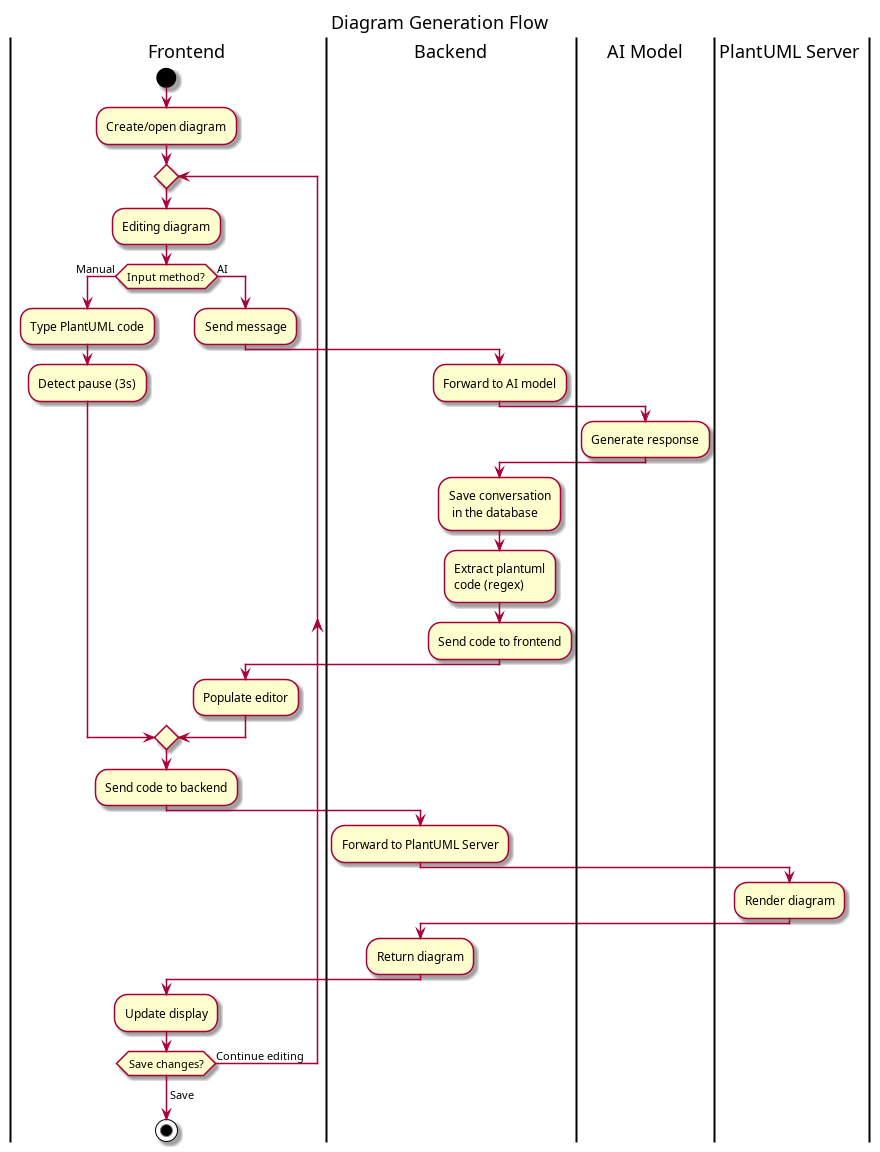
\includegraphics[width=0.8\textwidth]{conception/SprintIV/Activity_diagrams/edit_diagams.png}
\caption{Activity Diagram - Edit Diagrams}
\end{figure}

\subsection{Sequence Diagrams}

\begin{figure}[H]
\centering
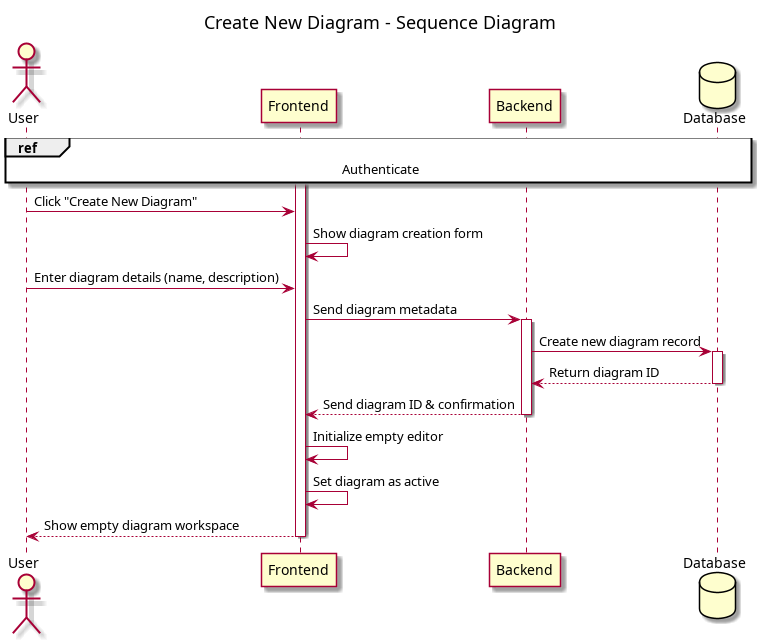
\includegraphics[width=0.8\textwidth]{conception/SprintIV/sequence_diagrams/sequence_diagramManagement_4_1_CreateNewDiagram.png}
\caption{Sequence Diagram - Create New Diagram}
\end{figure}

\begin{figure}[H]
\centering
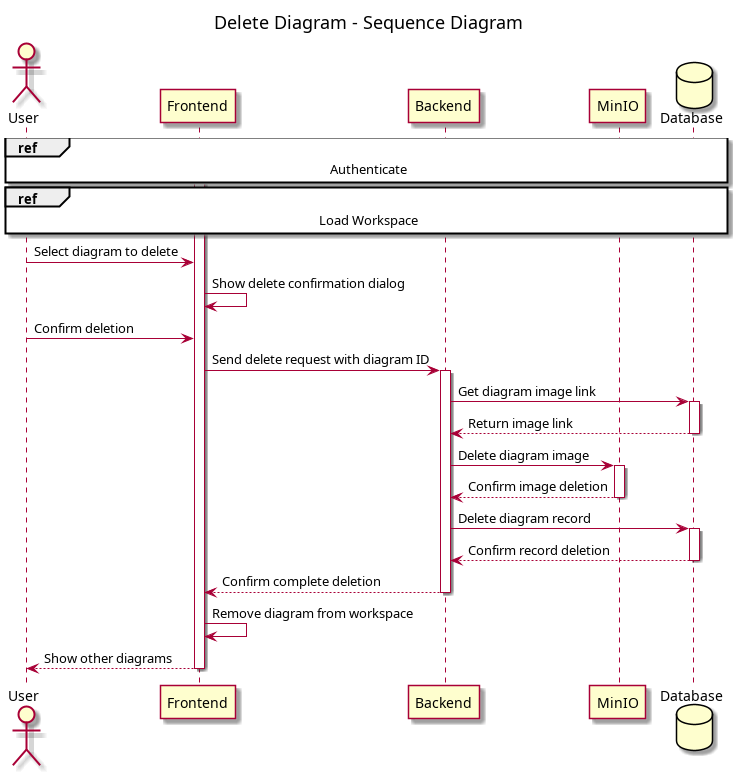
\includegraphics[width=0.8\textwidth]{conception/SprintIV/sequence_diagrams/sequence_diagramManagement_4_4_DeleteDiagram.png}
\caption{Sequence Diagram - Delete Diagram}
\end{figure}

\begin{figure}[H]
\centering
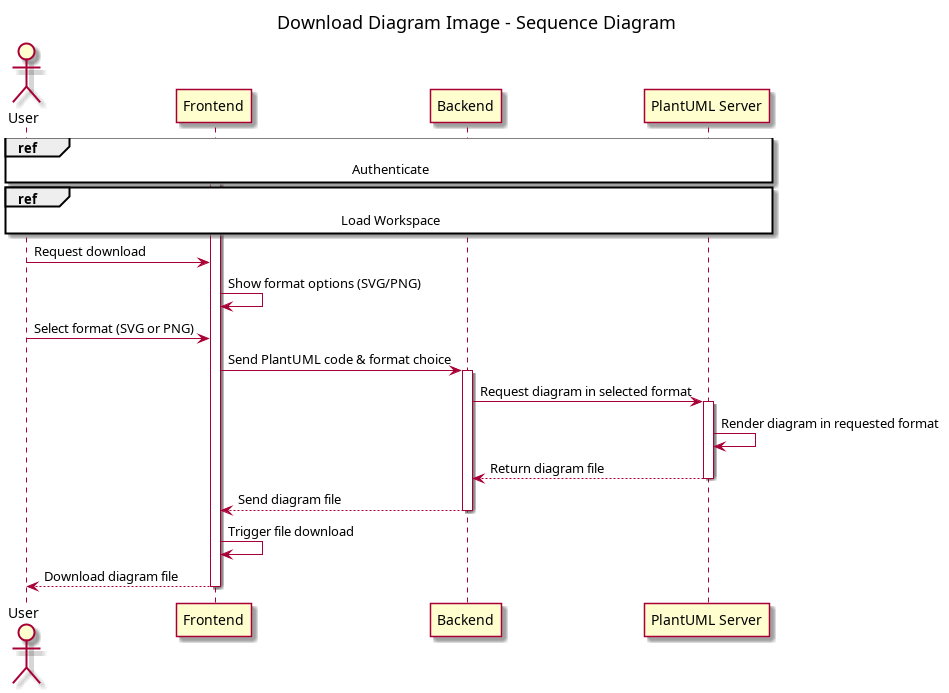
\includegraphics[width=0.8\textwidth]{conception/SprintIV/sequence_diagrams/sequence_workspaceManagement_4_5_DownloadDiagramImages.png}
\caption{Sequence Diagram - Download Diagram Images}
\end{figure}

\begin{figure}[H]
\centering
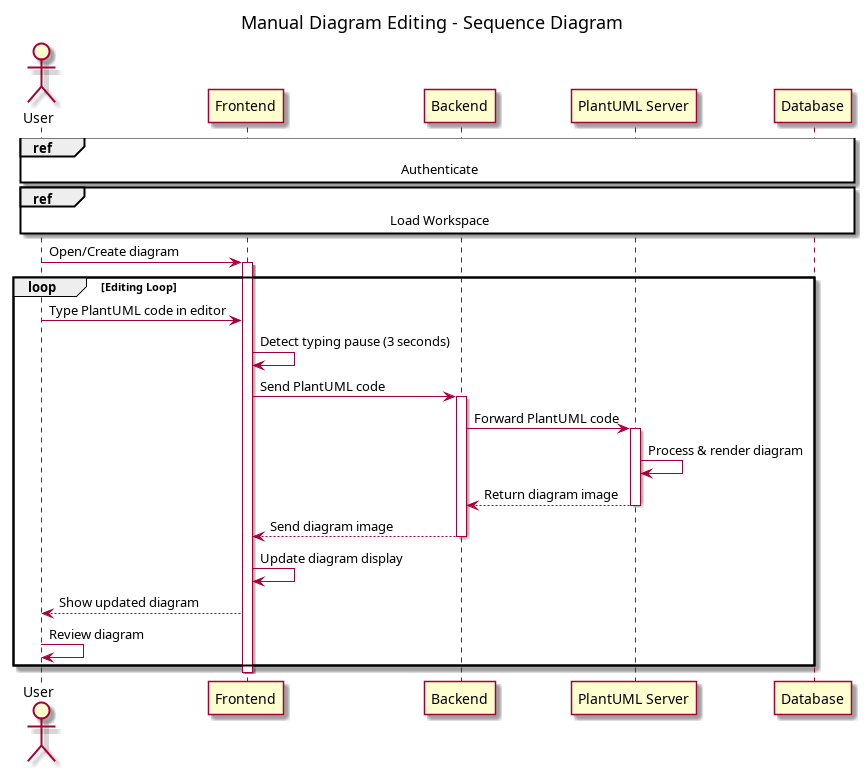
\includegraphics[width=0.8\textwidth]{conception/SprintIV/sequence_diagrams/sequence_workspaceManagement_5_2_EditDiagramCode.png}
\caption{Sequence Diagram - Edit Diagram Code}
\end{figure}

\begin{figure}[H]
\centering
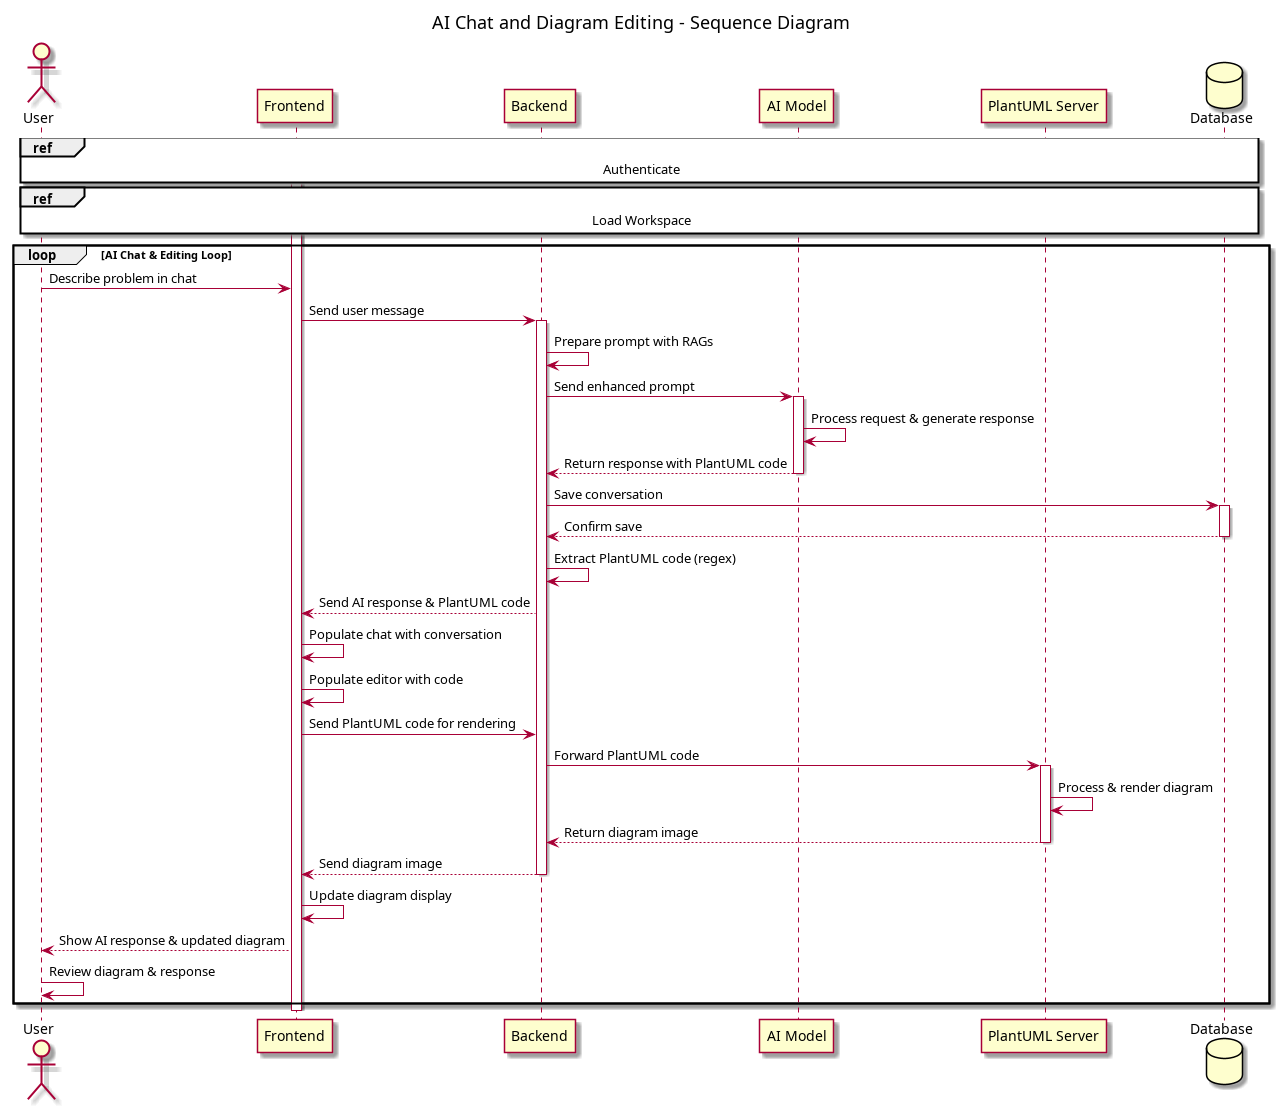
\includegraphics[width=0.8\textwidth]{conception/SprintIV/sequence_diagrams/sequence_workspaceManagement_5_3_ChatWithAIMode.png}
\caption{Sequence Diagram - Chat with AI Mode}
\end{figure}

\begin{figure}[H]
\centering
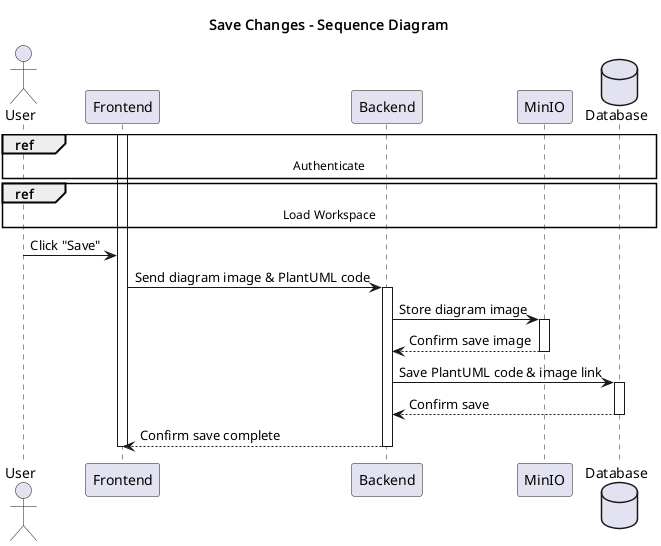
\includegraphics[width=0.8\textwidth]{conception/SprintIV/sequence_diagrams/sequence_workspaceManagement_save_changes.png}
\caption{Sequence Diagram - Save Changes}
\end{figure}

\section{Deliverables of Sprint IV}

Sprint IV delivered a comprehensive set of features that significantly enhance the user experience in diagram creation and management. The following screenshots demonstrate the key functionalities implemented during this sprint.

\begin{figure}[H]
\centering
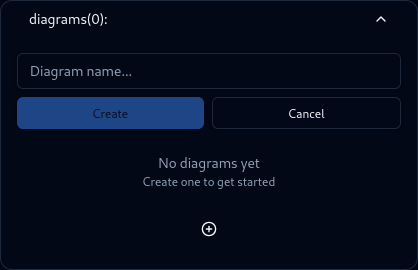
\includegraphics[width=0.8\textwidth]{screenshots/add-diagram.png}
\caption{Add Diagram Interface}
\end{figure}

The add diagram interface provides users with an intuitive way to create new diagrams. Users can specify diagram names, select diagram types, and initialize their diagramming projects efficiently.

\begin{figure}[H]
\centering
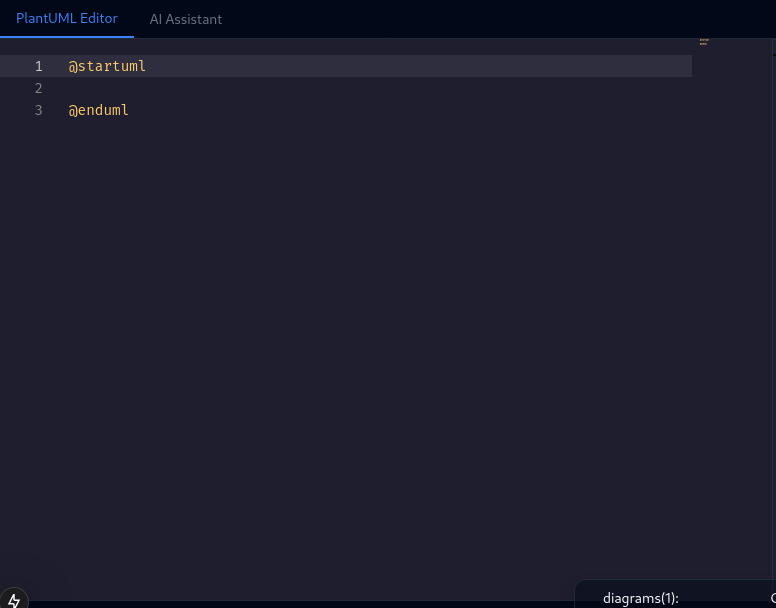
\includegraphics[width=0.8\textwidth]{screenshots/code-editor.png}
\caption{Interactive Code Editor}
\end{figure}

The interactive code editor serves as the primary workspace for diagram creation and editing. It features syntax highlighting, real-time validation, and seamless integration with the diagram preview functionality.

\begin{figure}[H]
\centering
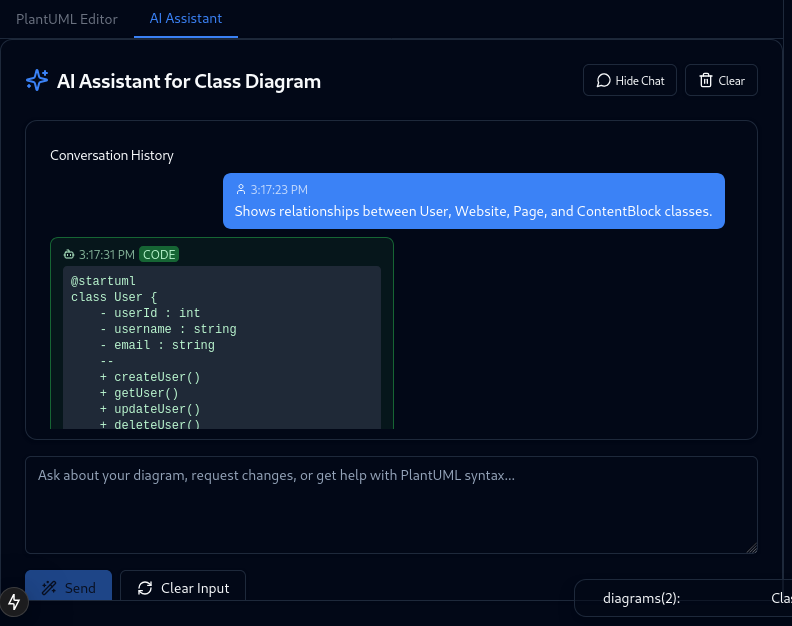
\includegraphics[width=0.8\textwidth]{screenshots/AI-assistant.png}
\caption{AI Assistant Integration}
\end{figure}

The AI assistant integration provides users with intelligent support for diagram creation and editing. Users can interact with the AI through natural language to receive suggestions, code improvements, and troubleshooting assistance.

\begin{figure}[H]
\centering
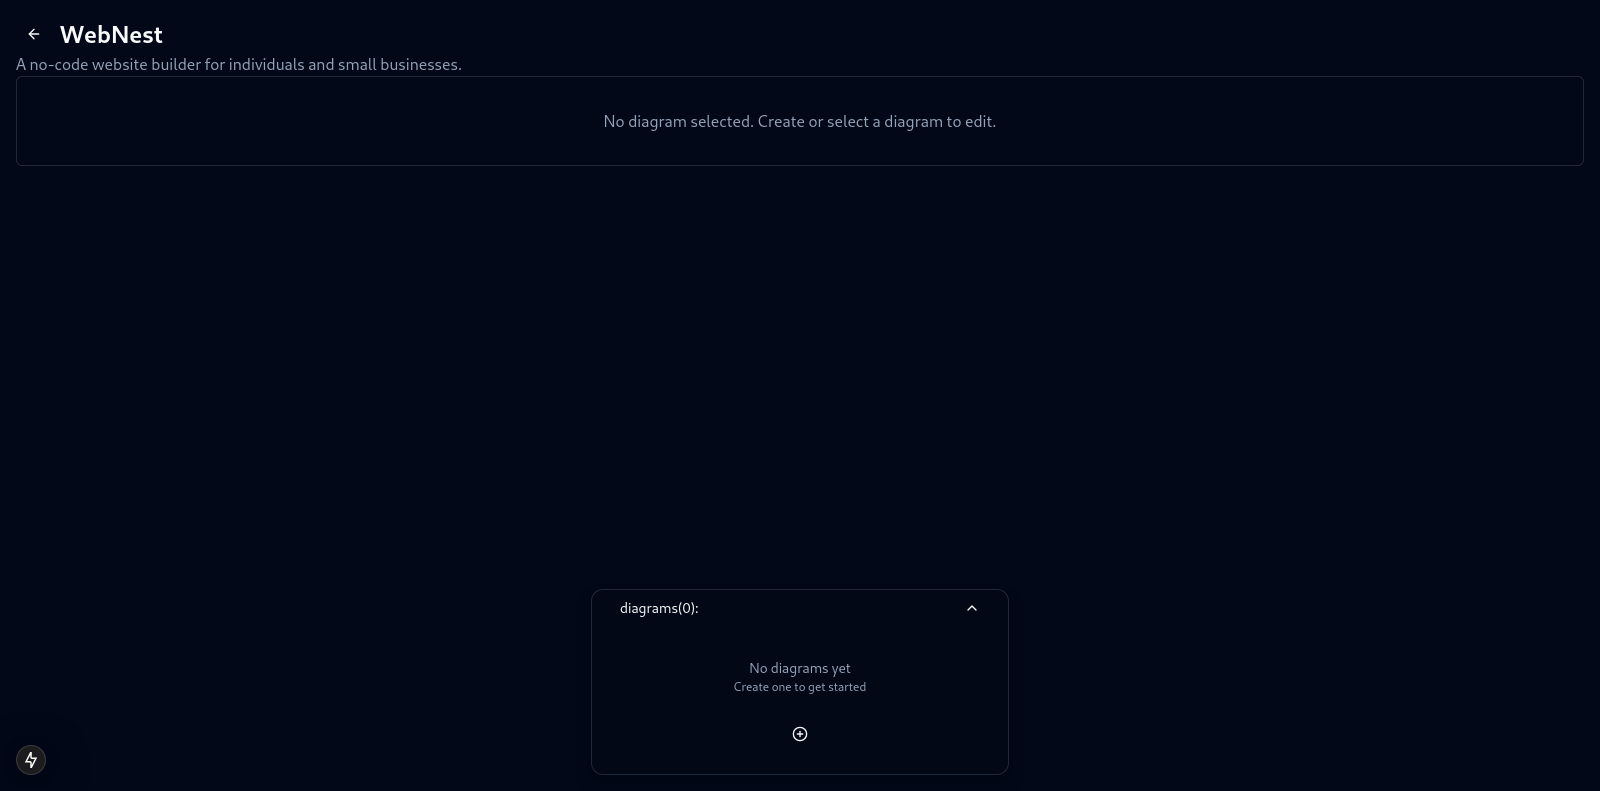
\includegraphics[width=0.8\textwidth]{screenshots/edit-diagram-project.png}
\caption{Diagram Project Editor - View 1}
\end{figure}

\begin{figure}[H]
\centering
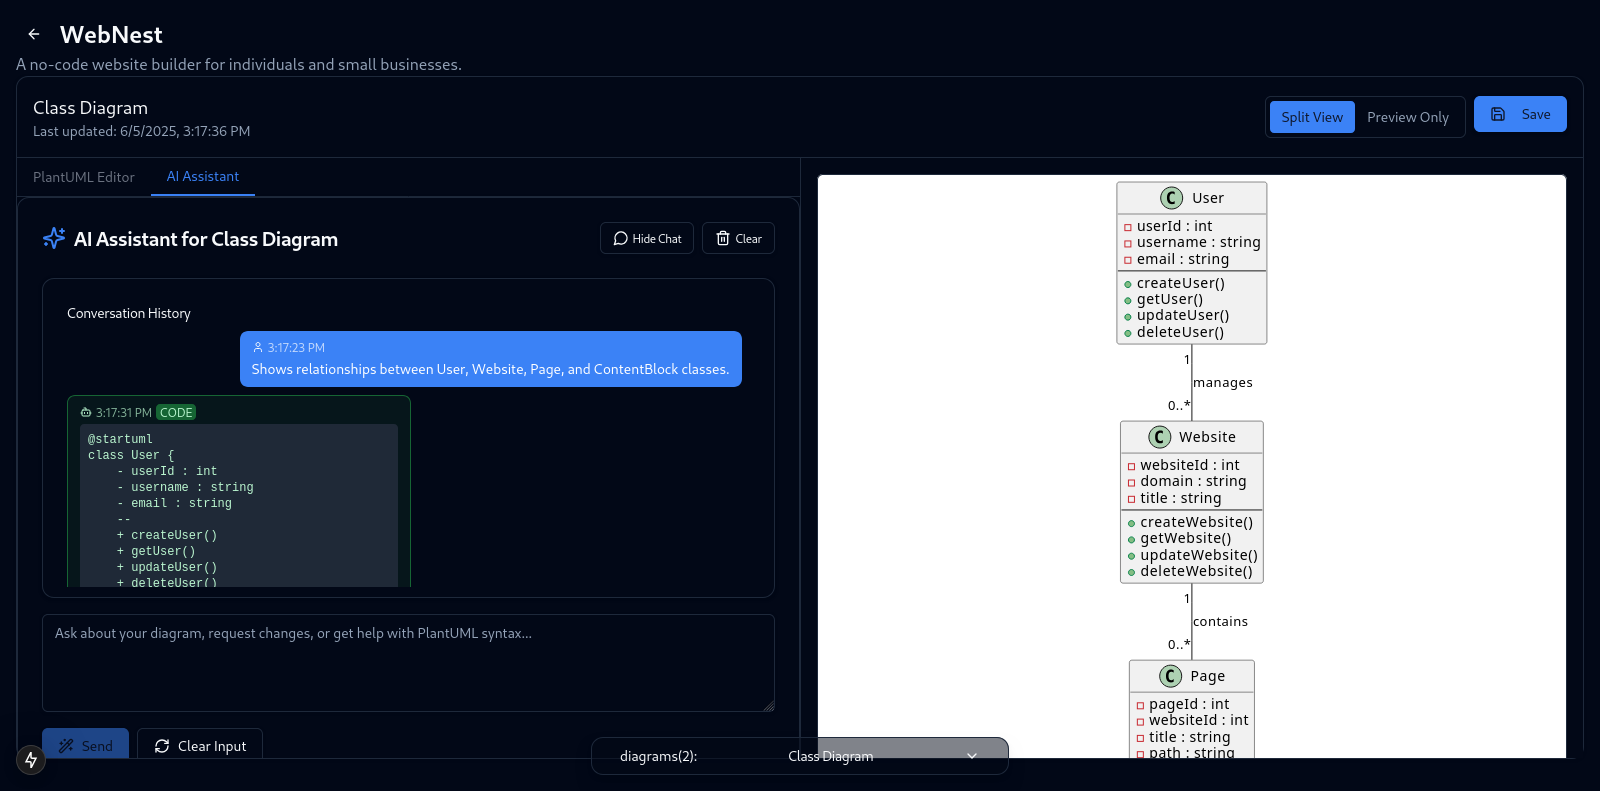
\includegraphics[width=0.8\textwidth]{screenshots/edit-diagram-project-2.png}
\caption{Diagram Project Editor - View 2}
\end{figure}

The diagram project editor showcases the split-view workspace functionality, allowing users to simultaneously edit code and preview diagrams. This dual-pane approach significantly improves productivity and provides immediate visual feedback for code changes.

\section{Retrospective of Sprint IV}

\begin{itemize}
\item \textbf{What went well:} Successful implementation of core diagram management CRUD operations, effective integration of AI assistant functionality, smooth PlantUML server integration for diagram rendering, positive user feedback on workspace split-view functionality
\item \textbf{Challenges faced:} Initial difficulties with AI service integration and response handling, performance optimization needed for large diagram rendering, browser compatibility issues with download functionality
\item \textbf{Areas for improvement:} Enhanced error handling for network failures, improved user interface responsiveness, better caching mechanisms for frequently accessed diagrams
\item \textbf{Lessons learned:} Importance of early AI service testing, need for comprehensive browser compatibility testing, value of user feedback in interface design decisions
\item \textbf{Action items for next sprint:} Implement advanced workspace customization features, enhance AI assistant capabilities, optimize application performance for large-scale diagrams
\end{itemize}

\section{Conclusion}

Sprint IV successfully delivered comprehensive diagram and workspace management capabilities that form the foundation of our diagramming application. The implementation of CRUD operations for diagrams, combined with an intelligent workspace featuring AI assistance and interactive editing, provides users with a powerful and intuitive platform for diagram creation and management. The integration of PlantUML server ensures high-quality diagram rendering, while the AI assistant adds significant value by providing intelligent support for complex diagramming tasks. The positive outcomes of this sprint establish a solid foundation for future enhancements and advanced features in subsequent development cycles.